% Manuscript v3 | 2026-09-27 | BDG selected; final comparative results pending.
% Build from paper/: pdflatex main; bibtex main; pdflatex main; pdflatex main.
% Previous live sources and PDF: versions/v2_pre_v3_2026-09-27/.
\documentclass{article}
\PassOptionsToPackage{numbers,compress}{natbib}
\usepackage[final,main]{neurips_2026}
\usepackage[utf8]{inputenc}
\usepackage[T1]{fontenc}
\usepackage{amsmath,amssymb,booktabs,graphicx,microtype,url}
\usepackage{algorithm,algpseudocode}
\usepackage{xcolor,tikz}
\usetikzlibrary{arrows.meta,positioning}
\usepackage{hyperref}
\hypersetup{hidelinks,pdftitle={BDG: Batch-Dispersion Guidance for Property-Band Generation},pdfsubject={Manuscript v3, 27 September 2026}}
\newcommand{\pend}{\textcolor{black!60}{\textsf{P}}}
\newcommand{\Fbar}{\bar F}
\newcommand{\Vb}{V_b}
\newcommand{\weff}{w_{\mathrm{eff}}}
\newcommand{\IB}{\mathrm{IB}}
\newcommand{\sg}{\operatorname{stopgrad}}
\title{BDG: Batch-Dispersion Guidance for\\Property-Band Generation}
\author{Bobo Li, Henry Huang, Idea Idehpour, Haimo Fang\\
Department of Computer and Information Science, University of Pennsylvania\\
\small Manuscript v3 \quad 27 September 2026}
\begin{document}
% MAIN_TEXT_START
\maketitle
\begin{abstract}
Continuous generative models learn to transport a simple reference distribution onto a complex data distribution, and their quality, controllability and transferability depend on the probability path, the training objective and the guidance rule. Property-targeted generation adds a requirement: samples must fall within a tolerance band around a target while retaining quality and diversity, and one guidance strength moves both a batch's centre and its spread. We introduce Batch-Dispersion Guidance (BDG), an inference-time rule that adjusts the deviation coefficient using the difference between the batch variance of predicted endpoint properties and a specified variance. BDG preserves the target-centering coefficient and uses the same network evaluations as plug-in guidance. We study it on QM9 molecular coordinates and on DeepFlyBrain DNA sequences on a probability simplex. The molecular study compares linear flow matching with variance-preserving diffusion under one matched protocol, compares guided with unguided sampling, and ablates the dispersion gain and setpoint; the rule then transfers unchanged to the simplex, where the state space, generator and property map differ. Algebraically, BDG reweights the plug-in direction through a batch-dependent gain and effective target, which bounds what the rule can reach. Final comparative results are pending, so improvements in band coverage, sample quality and transfer remain unresolved.
\end{abstract}

\section{Introduction}
Diffusion reverses a corruption process, and flow matching learns transport along a prescribed probability path \citep{karras2022elucidating,lipman2022flow}. Stochastic interpolants place both families under one construction \citep{albergo2025stochastic}, so a matched comparison is informative and not settled in advance.

Gradient guidance steers a frozen generator toward a target \citep{chung2023dps,song2023lgd}, and ensemble and moment constraints have precedent \citep{corso2024particle,mgd2026moment}; the open question is whether feedback from a learned endpoint property improves the quality--control trade-off.

We introduce BDG, study it on QM9 coordinates and DeepFlyBrain DNA simplices, and test whether adjusting dispersion separately from target centering improves band coverage at comparable quality on both state spaces. Our contributions are summarized as follows.
\begin{itemize}
\item We specify a paired molecular evaluation of the base models and guidance rules.
\item We define BDG and derive its relation to plug-in guidance and its widening condition.
\item We specify controls for dispersion gain, setpoint, strength, and feedback.
\item We implement the same scalar rule for sequences and specify how to assess transfer.
\end{itemize}

\section{Related Work}
\textbf{Continuous generation.} Flow matching fits conditional path velocities \citep{lipman2022flow}; diffusion design choices affect sampling quality and cost \citep{karras2022elucidating}. Stochastic interpolants and SiT unify the two families \citep{albergo2025stochastic,ma2024sit}, and rectified flow straightens the path \citep{liu2022flow}.

\textbf{Batch-dependent guidance.} Particle Guidance couples samples through a joint potential \citep{corso2024particle}, Moment Guided Diffusion targets prescribed moments \citep{mgd2026moment}, and Variance-Tilted Diffusion favors spread in a fixed linear feature space \citep{vtd2026variance}. Classifier-free and flow guidance scale one direction \citep{ho2022classifier,zheng2023guided}, whereas BDG reweights the deviation term by the residual between the empirical variance of endpoint property predictions and a user-set variance.

\textbf{Molecular comparisons.} Equivariant diffusion and EquiFM generate 3D molecules \citep{hoogeboom2022equivariant,song2023equifm}; DPS-style plug-in, LGD-MC, TMPD-inspired guidance and TFG steer a frozen generator \citep{chung2023dps,song2023lgd,boys2024tmpd,ye2024tfg}, with adaptations in Appendix~\ref{app:comparisons}.

\textbf{Sequence comparisons.} Dirichlet FM uses simplex paths, Fisher Flow categorical information geometry, and MOG-DFM guides sequence design \citep{stark2024dirichlet,davis2024fisher,chen2025multi}; these are the three planned external sequence comparators (Appendix~\ref{app:comparisons}).

\section{Methods}
\subsection{Modalities, Data, and Preprocessing}\label{sec:data}
QM9 \citep{ramakrishnan2014qm9} supplies centered coordinates with one-hot H/C/N/O/F types; the generator and guide $f_A$ train on one half of the molecules and the evaluator $f_B$ on the disjoint half, at targets $\mu$ (D), $\alpha$ (Bohr$^3$) and HOMO--LUMO gap (Ha) (Appendix~\ref{app:data}). DeepFlyBrain \citep{stark2024dirichlet} supplies 500-base-pair enhancers as A/C/G/T one-hot vectors on $(\Delta^3)^{500}$. Generation is unconditional in the property sense for both: $v_\theta$ takes no property or class input. Each sample draws its atom count as a mask $M$ from the training size histogram, so $M$ is the only conditioning variable and every arm shares it.

\subsection{Continuous Flow Matching Baseline}\label{sec:fm}
For data $x_1$, Gaussian source $x_0$, and $t\sim\mathcal U(0,1)$, the path and loss are
\begin{equation}
x_t=t x_1+(1-t)x_0,\qquad
\mathcal L_{\mathrm{FM}}=\mathbb E\|v_\theta(x_t,t;M)-(x_1-x_0)\|_M^2.
\label{eq:fm}
\end{equation}
Equation~\eqref{eq:fm} is the conditional flow-matching objective: the target is the velocity conditioned on the endpoint pair $(x_0,x_1)$, not on a property. The mask $M$ conditions the geometry through that norm and the induced graph; no property or class conditions the velocity. The norm, the E(3)-equivariant EGNN and the training budget are in Appendix~\ref{app:training}; sampling uses 100 Euler steps.

\subsection{Diffusion Baseline}\label{sec:diff}
The VP baseline matches the representation, split and network size. Noising time $u:0\to1$ gives $x_u=a(u)x_1+\sigma(u)\epsilon$ with projected Gaussian noise $\epsilon$, schedule $a(u)$ and $\sigma^2=1-a^2$, and $\epsilon_\phi$ minimises the masked noise MSE $\mathbb{E}\|\epsilon_\phi(x_u,u;M)-\epsilon\|_M^2$, written with its schedule in Equation~\eqref{eq:vp}. Sampling integrates the probability-flow ODE on a decreasing 100-step grid with terminal denoising, for 101 evaluations.

\subsection{Guided Generation}\label{sec:guidance}
For target $y$ and scale $s=f_A.\texttt{y\_std}>0$, plug-in guidance uses energy $(F_i-y)^2/(2s^2)$ at the endpoint estimate $m_i=x_t^{(i)}+(1-t)v_\theta(x_t^{(i)},t;M)$, with $F_i=f_A(m_i)$ and $J_i=\partial m_i/\partial x_t^{(i)}$. The field and clipped correction are
\begin{equation}
G_i=\frac{y-F_i}{s^2}J_i^\top\nabla_m f_A(m_i),\qquad
C_i=\operatorname{clip}_{\|v_i\|}\!\left(w\frac{1-t}{t}G_i\right).
\label{eq:plug}
\end{equation}
Here $\operatorname{clip}_r$ limits the correction norm to $r$; the generator and guide are frozen and $f_B$ only evaluates.

\subsection{Proposed Innovation: Batch-Dispersion Guidance}\label{sec:bdg}
The weakness is that plug-in guidance derives its coefficient from one quadratic energy, so a single strength moves a batch's centre and shrinks its spread together, coupling coverage to contraction. We hypothesize that giving the deviation term its own coefficient decouples them. For $B\ge2$, define $\Fbar=B^{-1}\sum_iF_i$, $\Vb=(B-1)^{-1}\sum_i(F_i-\Fbar)^2$, and $\tau=\tau_{\mathrm{mult}}s>0$. Replace $y-F_i$ in Equation~\eqref{eq:plug} with
\begin{equation}
n_i=(y-F_i)-\eta e(F_i-\Fbar)=(y-\Fbar)-\weff(F_i-\Fbar),\qquad
e=\frac{\Vb-\tau^2}{\tau^2},\quad \weff=1+\eta e.
\label{eq:bdg}
\end{equation}
The gain $\eta\ge0$ changes only the deviation coefficient. Positive $e$ strengthens contraction and negative $e$ weakens it; net repulsion requires $\weff<0$, that is $\eta>1$ and $\Vb<\tau^2(1-1/\eta)$. BDG retains the plug-in direction with a state-dependent gain and effective target (Algorithm~\ref{alg:bdg}, Appendix~\ref{app:algebra}). Three controls isolate the innovation: $\eta=0$ must reproduce plug-in exactly, a matched-strength plug-in separates dispersion from strength, and an open-loop replay separates feedback from schedule (Section~\ref{sec:ablations}).

\subsection{Transfer to Modality 2}\label{sec:transfer}
The sequence model uses a linear path from a Dirichlet$(1,1,1,1)$ source and retains Equation~\eqref{eq:bdg}, with soft GC fraction and CpG frequency in place of the learned guide; simplex projection enforces feasibility (Appendix~\ref{app:m2}).

\subsection{Model Overview}\label{sec:overview}
Figure~\ref{fig:overview}(a) carries the QM9 chain, where BDG changes one term in the sampling step and nothing else; panel~(b) is the transfer.

\begin{figure}[!t]
\centering
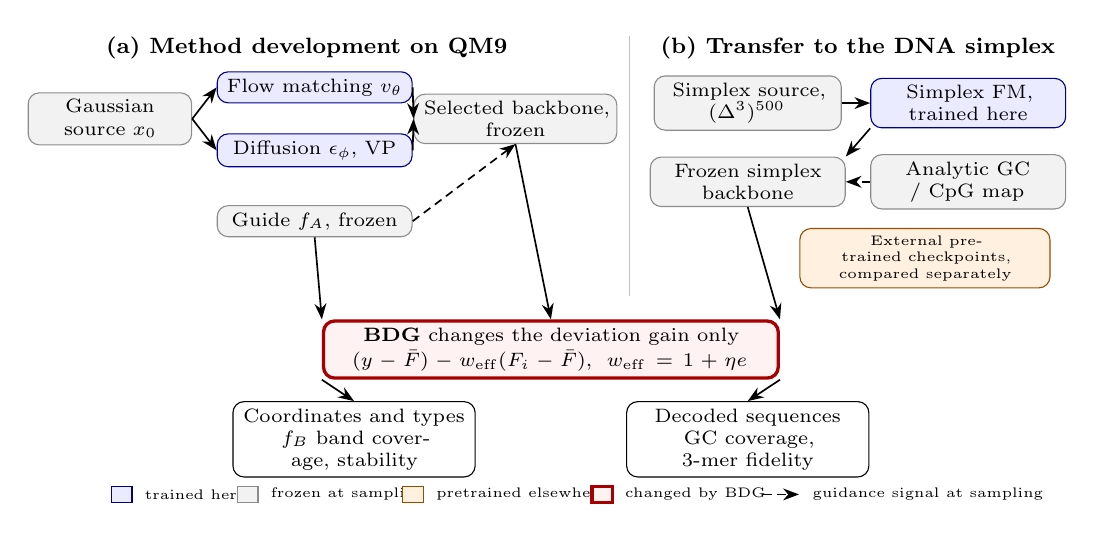
\begin{tikzpicture}[font=\scriptsize,
  box/.style={draw,rounded corners,align=center,inner sep=2.5pt},
  trained/.style={box,fill=blue!8,draw=blue!55!black},
  frozen/.style={box,fill=black!5,draw=black!45},
  pre/.style={box,fill=orange!12,draw=orange!60!black},
  innov/.style={box,fill=red!5,draw=red!65!black,very thick},
  arr/.style={-{Stealth},semithick},
  gsig/.style={-{Stealth},semithick,densely dashed},
  key/.style={draw,minimum width=0.26cm,minimum height=0.2cm,inner sep=0}]

% ---- panel (a) : development on QM9
\node[font=\footnotesize\bfseries] at (0.3,2.05) {(a) Method development on QM9};
\node[frozen,text width=1.9cm] (src) at (-2.2,1.15) {Gaussian source $x_0$};
\node[trained,text width=2.3cm] (fm)  at (0.4,1.55) {Flow matching $v_\theta$};
\node[trained,text width=2.3cm] (vp)  at (0.4,0.75) {Diffusion $\epsilon_\phi$, VP};
\node[frozen,text width=2.4cm] (sel)  at (2.95,1.15) {Selected backbone,\\frozen};
\node[frozen,text width=2.3cm] (guide) at (0.4,-0.15) {Guide $f_A$, frozen};
\draw[arr] (src.east)--(fm.west);
\draw[arr] (src.east)--(vp.west);
\draw[arr] (fm.east)--(sel.west);
\draw[arr] (vp.east)--(sel.west);
\draw[gsig] (guide.east)--(sel.south);

% ---- divider
\draw[black!25] (4.4,2.2)--(4.4,-1.1);

% ---- panel (b) : transfer to the simplex
\node[font=\footnotesize\bfseries] at (7.3,2.05) {(b) Transfer to the DNA simplex};
\node[frozen,text width=2.2cm] (src2)  at (5.9,1.35) {Simplex source, $(\Delta^3)^{500}$};
\node[trained,text width=2.3cm] (sfm)   at (8.7,1.35) {Simplex FM, trained here};
\node[frozen,text width=2.3cm] (sel2)  at (5.9,0.35) {Frozen simplex\\backbone};
\node[frozen,text width=2.3cm] (prop2) at (8.7,0.35) {Analytic GC / CpG map};
\draw[arr] (src2.east)--(sfm.west);
\draw[arr] (sfm.south west)--(sel2.north east);
\draw[gsig] (prop2.west)--(sel2.east);
\node[pre,text width=3.0cm,font=\tiny] (ext) at (8.15,-0.62)
  {External pretrained checkpoints,\\compared separately};

% ---- the shared rule
\node[innov,text width=5.6cm] (bdg) at (3.4,-1.78)
  {\textbf{BDG} changes the deviation gain only\\[1pt]
   $(y-\Fbar)-\weff(F_i-\Fbar)$, \ $\weff=1+\eta e$};
\draw[arr] (guide.south)--(bdg.north west);
\draw[arr] (sel.south)--(bdg.north);
\draw[arr] (sel2.south)--(bdg.north east);

% ---- outputs
\node[box,text width=2.9cm] (o1) at (0.9,-2.92) {Coordinates and types\\$f_B$ band coverage, stability};
\node[box,text width=2.9cm] (o2) at (5.9,-2.92) {Decoded sequences\\GC coverage, 3-mer fidelity};
\draw[arr] (bdg.south west)--(o1.north);
\draw[arr] (bdg.south east)--(o2.north);

% ---- key
\node[key,fill=blue!8,draw=blue!55!black] at (-2.05,-3.62) {};
\node[anchor=west,font=\tiny] at (-1.88,-3.62) {trained here};
\node[key,fill=black!5,draw=black!45] at (-0.45,-3.62) {};
\node[anchor=west,font=\tiny] at (-0.28,-3.62) {frozen at sampling};
\node[key,fill=orange!12,draw=orange!60!black] at (1.65,-3.62) {};
\node[anchor=west,font=\tiny] at (1.82,-3.62) {pretrained elsewhere};
\node[key,fill=red!5,draw=red!65!black,very thick] at (4.05,-3.62) {};
\node[anchor=west,font=\tiny] at (4.22,-3.62) {changed by BDG};
\draw[gsig] (6.1,-3.62)--(6.55,-3.62);
\node[anchor=west,font=\tiny] at (6.6,-3.62) {guidance signal at sampling};
\end{tikzpicture}
\caption{Overview of the study. \textbf{(a)} Method development on QM9: one source, the two families we train, the matched comparison that selects and freezes the backbone, and the frozen guide supplying the property gradient at sampling time (dashed). BDG replaces the deviation gain only. \textbf{(b)} Transfer to the simplex. External pretrained checkpoints are never pooled with models trained here.}
\label{fig:overview}
\end{figure}

\section{Results}
\subsection{Evaluation Protocol}\label{sec:protocol}
The protocol is fixed before interpretation; \pend{} marks a pending value in Tables~\ref{tab:fmvd}--\ref{tab:m2}.

\subsubsection{Metrics}
On QM9, controllability is band coverage $\IB=n^{-1}\sum_i\mathbf1\{|f_B(\hat x_i)-y|\le\delta\}$ on decoded samples, at median training target $y$ with $\delta=2\operatorname{MAE}_{\mathrm{cal}}(f_B)$; fidelity is molecule stability and RDKit validity; diversity is uniqueness and distinct-valid yield. IB inherits $f_B$'s error, so a guided arm can raise it by exploiting the evaluator. On the DNA simplex, fidelity is decoded validity and 3-mer fidelity, diversity is pairwise distinctness, and controllability is GC-band coverage under the exact count, which carries no evaluator error but is coarse, and we do not quote the standard enhancer classifier (Appendix~\ref{app:m2}).

\subsubsection{Fair Comparison and Computational Budget}
The two baselines share split, preprocessing, conditioning, atom-count mask, evaluator and metrics, differing only in the corruption process, at 100 and 101 evaluations. Per-cell settings, budgets and hardware are fixed in Appendices~\ref{app:training} and~\ref{app:evaluation}. Two mismatches remain: equal $w$ is equal nominal strength, not equal applied force; and external baselines run from released checkpoints, so they stay inside their own backend (Table~\ref{tab:backends}).

\subsubsection{Statistical Reporting}
Every principal result reports seed means, standard deviations and paired per-seed differences over three seeds. BDG couples samples through $\Fbar$ and $\Vb$, so the batch is the unit of uncertainty. All arms stay visible, no chemistry threshold removes a result, and produced numbers are labelled separately from quoted ones.

\subsection{Modality 1: Flow Matching versus Diffusion}\label{sec:fmvd}
The Methods are written on the flow backbone, which Table~\ref{tab:fmvd} must support on quality and cost jointly, not on one metric; otherwise the guidance sections re-instantiate unchanged on the VP ODE.

\begin{table}[!htbp]
\centering\small
\caption{Matched QM9 base models, as seed mean $\pm$ standard deviation of fractions. NFE includes terminal denoising.}
\label{tab:fmvd}
\begin{tabular}{lccccc}
\toprule
Model & Mol. stab.$\uparrow$ & Validity$\uparrow$ & Uniqueness$\uparrow$ & NFE$\downarrow$ & Time$\downarrow$\\
\midrule
FM, trained here & \pend & \pend & \pend & 100 & \pend\\
VP, trained here & \pend & \pend & \pend & 101 & \pend\\
\bottomrule
\end{tabular}
\end{table}


\subsection{Modality 1: Guided versus Unguided Generation}\label{sec:guidworks}
The paired comparison will test target improvement and chemistry cost (Table~\ref{tab:guidance}).

\begin{table}[!htbp]
\centering\small
\caption{QM9 guidance against a matched unguided control, by property. $w$ is nominal guidance strength; DV is distinct-valid molecules per attempt. The headline uses $w=1$; $w=4$ shows the trade-off.}
\label{tab:guidance}
\begin{tabular}{lcccccc}
\toprule
Arm & $w$ & IB$\uparrow$ & Mol. stab.$\uparrow$ & Validity$\uparrow$ & Uniqueness$\uparrow$ & DV$\uparrow$\\
\midrule
Unguided & $0$ & \pend & \pend & \pend & \pend & \pend\\
Plug-in & $1$ & \pend & \pend & \pend & \pend & \pend\\
Plug-in & $4$ & \pend & \pend & \pend & \pend & \pend\\
\bottomrule
\end{tabular}
\end{table}


\subsection{Modality 1: Innovation Ablations}\label{sec:ablations}
The registered grid sweeps gain and setpoint at $w\in\{1,4\}$, with one $\eta=0$ setting (Appendix~\ref{app:evaluation}); Table~\ref{tab:ablation} identifies the controls, and clipping frequency and realized gain must accompany attribution to dispersion.

\begin{table}[!htbp]
\centering\small
\caption{BDG controls. $\Delta$IB is the paired change from plug-in; $R$ is decoded property standard deviation divided by unguided.}
\label{tab:ablation}
\begin{tabular}{llccc}
\toprule
Control & Effect isolated & $\Delta$IB & $R$ & Mol. stab.$\uparrow$\\
\midrule
$\eta=0$ & identity to plug-in & \pend & \pend & \pend\\
Gain/setpoint, $w=1,4$ & dispersion vs. strength & \pend & \pend & \pend\\
One-sided residual & negative-residual branch & \pend & \pend & \pend\\
Open-loop replay & feedback vs. schedule & \pend & \pend & \pend\\
Signed-strength plug-in & scalar reweighting & \pend & \pend & \pend\\
\bottomrule
\end{tabular}
\end{table}


\subsection{Modality 1: Comparison with Recent Methods}\label{sec:recent}
Table~\ref{tab:recent} reserves four recent guidance comparisons per flow backend, since property pairs and acceptance widths differ (costs in Appendix~\ref{app:evaluation}).

\begin{table}[!htbp]
\centering\small
\caption{Molecular guidance at $w=1$, per property and backend. BDG uses $\eta=4$ and $\tau_{\mathrm{mult}}=0.5,1.0$, reported separately. Prior-method rows are adaptations.}
\label{tab:recent}
\begin{tabular}{lcccc}
\toprule
Method & IB$\uparrow$ & Mol. stab.$\uparrow$ & DV$\uparrow$ & Time$\downarrow$\\
\midrule
Unguided, selected backbone & \pend & \pend & \pend & \pend\\
\midrule
DPS-style plug-in \citep{chung2023dps} & \pend & \pend & \pend & \pend\\
TMPD-inspired \citep{boys2024tmpd} & \pend & \pend & \pend & \pend\\
LGD-MC \citep{song2023lgd} & \pend & \pend & \pend & \pend\\
TFG \citep{ye2024tfg} & \pend & \pend & \pend & \pend\\
BDG (ours) & \pend & \pend & \pend & \pend\\
\bottomrule
\end{tabular}
\end{table}


\subsection{Modality 2: Transfer of the Innovation}\label{sec:m2}
Sequence evaluation pairs exact GC/CpG band coverage with 3-mer JSD and diversity (Table~\ref{tab:m2}).

\begin{table}[!htbp]
\centering\small
\caption{Planned DeepFlyBrain comparisons at length 500, by property. JSD measures 3-mer mismatch; diversity is mean normalized pairwise Hamming distance.}
\label{tab:m2}
\begin{tabular}{lcccc}
\toprule
Method & IB$\uparrow$ & JSD$\downarrow$ & Diversity$\uparrow$ & Time$\downarrow$\\
\midrule
Simplex FM, unguided & \pend & \pend & \pend & \pend\\
Simplex FM + plug-in & \pend & \pend & \pend & \pend\\
Simplex FM + BDG & \pend & \pend & \pend & \pend\\
Dirichlet FM \citep{stark2024dirichlet} & \pend & \pend & \pend & \pend\\
Fisher Flow \citep{davis2024fisher} & \pend & \pend & \pend & \pend\\
MOG-DFM \citep{chen2025multi} & \pend & \pend & \pend & \pend\\
\bottomrule
\end{tabular}
\end{table}


\subsection{Cross-Modality Analysis and Failure Modes}\label{sec:failure}
Predictor error can separate guided from evaluated molecular properties, and sequence relaxation and decoding can create a similar mismatch. We compare each modality's BDG-minus-plug-in change, in sign and size, against its own baseline, and ask whether the residual acts through the same contraction term in both. The central question is unanswered: implementation and algebra are settled, coverage and transfer are not.

\section{Discussion}
BDG adds a dispersion residual to the guidance coefficient, separating target centering from deviation weighting and identifying when the latter turns repulsive.

Final measurements must decide coverage, quality, the controls and transfer; model selection, predictor reliability and unmatched external evaluation bound any stronger conclusion.

Two limitations shape the next steps. A held-out predictor scores band coverage, so an arm can gain by exploiting evaluator error; a second independent evaluator would settle that. Clipping and projection alter the analysed correction; the per-cell log of Section~\ref{sec:ablations} would settle that. The narrowest supported claim is that a dispersion residual changes the deviation coefficient as derived, on two state spaces, under one protocol.
% MAIN_TEXT_END
\clearpage
\bibliographystyle{ieeetr}
\bibliography{citation,refs_extra}
\clearpage
\appendix
\renewcommand{\thetable}{S\arabic{table}}
\setcounter{table}{0}
\renewcommand{\thefigure}{S\arabic{figure}}
\setcounter{figure}{0}
\section{Reproducibility and Extended Protocol}
\subsection{Data Sources and Splits}\label{app:data}
The QM9 source is the DeepChem/MoleculeNet packaging. The project retains the 3{,}054 entries removed as uncharacterized in common EDM preprocessing, so its data definition differs from those benchmarks. A seeded permutation creates the splits: 51{,}527 molecules in \texttt{train\_a}, a disjoint 51{,}527 in \texttt{train\_b}, 17{,}748 validation and 13{,}083 test. Centering removes translation; predictors are invariant. Coordinates and one-hot types have no additional scaling. Predictors use training-derived property normalization. Molecular sizes are paired across arms within each backend.

DeepFlyBrain is stored in \path{proj1/m2/blade_bundle/dfb500.npz}. Four ambiguous training examples were excluded from the supplied 83{,}726. The channel order is A/C/G/T and length is 500, and the retained train/validation/test counts are 83{,}722/10{,}505/10{,}434. Cell-type labels are not supplied to our unconditional generator. Random-example splits do not establish sequence-cluster or out-of-distribution generalization. The older 200-base-pair Kenyon-cell setup is excluded from the final comparison.

\subsection{Training and Checkpoint Records}\label{app:training}
Table~\ref{tab:training} separates configurations from final provenance. Matching configurations does not establish equal completed training. Checkpoints, actual epochs, and selection rules must accompany FM--VP evaluation. The existing FM record uses final EMA weights; VP code selects by validation generation stability with loss as tie-breaker. This difference must be disclosed or aligned before selection.

\begin{table}[!htbp]
\centering\small
\caption{Training configuration and recorded properties. Asterisks mark configured settings requiring final run verification. P denotes missing final provenance. Predictor counts are per property network.}
\label{tab:training}
\begin{tabular}{llll}
\toprule
Setting & Molecular FM / VP & $f_A$ / $f_B$ & Sequence FM\\
\midrule
Architecture & EGNN, 256, 8 layers & invariant EGNN, 128, 4 & CNN, 128, 10 layers\\
Parameters & 3.75 M each & 429{,}825 each & approximately 1.02 M\\
Training split & \texttt{train\_a} & \texttt{train\_a} / \texttt{train\_b} & DeepFlyBrain train\\
Objective & velocity / noise MSE & property MSE & velocity MSE\\
Epochs & 1{,}500$^*$ & 120 & 1{,}500 recorded\\
Batch & 256$^*$ & 128 & 256\\
Optimizer & Adam$^*$ & Adam & \pend\\
Learning rate & $2\times10^{-4}$, cosine$^*$ & $3\times10^{-4}$, cosine & $2\times10^{-3}$, cosine\\
EMA & 0.9999$^*$ & none & \pend\\
Run seed & 20260918$^*$ & \pend & \pend\\
Hashes / hardware & \pend & \pend & \pend\\
\bottomrule
\end{tabular}
\end{table}

For coordinates $c$ and features $f$, the norm in Equations~\eqref{eq:fm} and~\eqref{eq:vp} is
\[
\|z\|_M^2=\frac{\|M\odot z^c\|_2^2}{3\sum M}+\frac{\|M\odot z^f\|_2^2}{5\sum M}.
\]
The mask $M$ broadcasts over channels. Coordinate noise is projected to zero center of mass, giving dimension $3(N-1)$ for $N$ atoms. Feature noise is Gaussian. Atom types use the largest final feature component. VP time $u$ is clean-to-noise; flow time $t$ is noise-to-data.

The VP process and loss of Section~\ref{sec:diff} are
\begin{equation}
\begin{aligned}
x_u&=a(u)x_1+\sigma(u)\epsilon,\quad a(u)=e^{-\frac12(0.1u+9.95u^2)},\quad \sigma^2=1-a^2,\\
\mathcal L_{\mathrm{VP}}&=\mathbb E\|\epsilon_\phi(x_u,u;M)-\epsilon\|_M^2,
\end{aligned}
\label{eq:vp}
\end{equation}
with $\beta(u)=0.1+19.9u$ and probability-flow ODE $\mathrm dx/\mathrm du=-\tfrac12\beta(u)(x+s_\phi)$, where $s_\phi=-\epsilon_\phi/\sigma$. QM9 preprocessing keeps coordinates and one-hot types unscaled, and the dataset supplies 133{,}885 molecules before splitting.

\subsection{Evaluation and Cost Accounting}\label{app:evaluation}
The molecular protocol fixes seeds 20261001, 20261002, and 20261003, q50 targets, $w=1$, $t_{\min}=0.5$, and batch 500. Per-cell $n$ is operator-selected and divisible by 500. Each cell runs $n/500$ separately coupled batches. Increasing $n$ adds batches without changing each variance estimator's sample count. Batch size is a BDG design parameter.

The calibration pool contains 3{,}000 molecules from the two training halves. Internal predictors are calibrated only on the half they did not train on. Evaluator-specific acceptance widths differ from $\tau=\tau_{\mathrm{mult}}f_A.\texttt{y\_std}$. Final cells record widths and predictor identities (Table~\ref{tab:backends}).

\begin{table}[!htbp]
\centering\small
\caption{Molecular guidance backends. External generators are pretrained and frozen. Results stay within backend. External EDM is separate from our trained VP comparison.}
\label{tab:backends}
\begin{tabular}{lll}
\toprule
Generator & Guide / evaluator & Headline arms\\
\midrule
Our FM & internal disjoint pair & all seven\\
External EquiFM & released TFG pair & all seven\\
External EDMsecond & internal disjoint pair & unguided, plug-in\\
\bottomrule
\end{tabular}
\end{table}

The seven arms are unguided, plug-in, TMPD-inspired, LGD-MC, TFG, and BDG at $\eta=4$, $\tau_{\mathrm{mult}}\in\{0.5,1\}$. The registered ablation grid is $\eta\in\{1,2,4,8\}$ and $\tau_{\mathrm{mult}}\in\{0.5,0.75,1,1.5\}$, with one $\eta=0$ setting, at $w\in\{1,4\}$. Two setpoints cannot establish a monotone curve; the ablation supplies additional gains and setpoints. All arms remain visible regardless of stability. The pilot chemistry floor does not govern this protocol.

Atom stability is the fraction satisfying the project's bond/valence rules; molecule stability requires all atoms to pass. RDKit validity uses fixed reconstruction and sanitization. Uniqueness divides distinct canonical SMILES by valid samples; distinct-valid yield divides distinct valid molecules by all attempts. Stability and validity are bond-table conventions, not energies, and uniqueness saturates near one at this scale. We will report attempted, decoded, valid, and distinct-valid counts, and every guided arm reports the metric guidance optimises beside one it does not. Band coverage includes chemically invalid samples and cannot alone measure usable yield.

We distinguish $f_A$ endpoint spread as a controller diagnostic from $f_B$ decoded spread as an evaluation diagnostic. Neither equals structural diversity. The analysis will report three seed values, mean, sample standard deviation, and paired changes under common noise. Intervals must respect coupled batches. Sampling seeds quantify sampling variation at fixed weights, not training-seed uncertainty.

Cost accounting will include generator forwards, generator vector--Jacobian products, guide forwards/backwards, peak memory, and seconds per sample on matched hardware. BDG adds reductions to plug-in's calls; equal calls do not establish equal runtime. Final manifests will supply Monte Carlo counts and optimization steps.

\subsection{Baseline Adaptations and Comparison Limits}\label{app:comparisons}
Our DPS-style plug-in adapts inverse-problem guidance to a Gaussian property energy and flow endpoint. TMPD-inspired guidance linearizes property uncertainty. LGD-MC and TFG also require disclosed endpoint, noise, and sampler choices. These adaptations do not reproduce every published benchmark.

External EquiFM and EDMsecond differ from our FM--VP pair in data, architecture, and parameterization. EquiFM uses TFG predictors with different acceptance widths and uncertain training overlap. Coverage comparisons stay within backend and predictor pair.

Dirichlet FM, Fisher Flow, and MOG-DFM require common length, target, band width, conditioning, decoding, and reference data. Published class-conditioned scores do not establish GC/CpG-band performance. These rows are pending evaluations. Guidance ports on our sequence generator do not themselves reproduce these three models.

\subsection{Sequence Transfer Protocol}\label{app:m2}
The shipped model is \path{proj1/m2/blade_bundle/fm_m2_dfb500.pt}. Its path joins a uniform Dirichlet source to one-hot sequences. The sampler clamps each Euler update to nonnegative values, renormalizes per position, and decodes by $\arg\max$. Endpoint extrapolation used by the guide need not lie on the simplex, creating a possible mismatch with decoded counts.

For relaxed sequence $p\in\mathbb R^{L\times4}$,
\[
F_{\mathrm{GC}}(p)=L^{-1}\sum_{j=1}^L(p_{j,C}+p_{j,G}),\qquad
F_{\mathrm{CpG}}(p)=(L-1)^{-1}\sum_{j=1}^{L-1}p_{j,C}p_{j+1,G}.
\]
GC is affine; CpG is quadratic. Evaluation counts bases or adjacent pairs after decoding. Exact counts have no prediction error to define a nonzero band. Existing code uses $\delta=\max(0.16s,4.4/(L-1))$, with training-property standard deviation $s$. GC/CpG counting increments are $1/L$ and $1/(L-1)$; the current floor uses the latter for both. Final widths must be fixed before comparison and are not commensurate with molecular bands.

Final sequence timing, batch size, $n$, seeds, and comparator alignment remain unspecified. The driver defaults to $t_{\min}=0$; earlier pilots used $0.5$. Sequence timing and batch size remain unresolved. Table~\ref{tab:m2} requires one declared protocol.

Three-mer JSD compares generated and held-out frequencies. Diversity is mean normalized pairwise Hamming distance, with the pair-sampling rule recorded. Evaluation will also include decoding confidence and duplicates. Composition statistics do not establish enhancer activity or cell-type specificity.

\subsection{BDG Algorithm and Algebraic Limits}\label{app:algebra}
Algorithm~\ref{alg:bdg} gives the update. All weights are fixed. Batch statistics determine coefficients; the pullback differentiates properties with coefficients held fixed. Differentiating a loss through the coefficients would produce another update.

\begin{algorithm}[htbp]
\caption{One BDG-guided Euler step}\label{alg:bdg}
\begin{algorithmic}[1]
\Require batch $x_t$, frozen $v_\theta$ and $f$, target $y$, scale $s>0$, gain $\eta\ge0$, setpoint $\tau>0$, strength $w$, step $h$, start $t_{\min}$
\State $v\gets v_\theta(x_t,t;M)$
\If{$t<t_{\min}$} \State \Return $\Pi(x_t+h v)$ \EndIf
\State $m\gets x_t+(1-t)v_\theta(x_t,t;M)$ with gradients enabled
\State $F_i\gets f(m_i)$; $\Fbar\gets B^{-1}\sum_iF_i$
\State $\Vb\gets (B-1)^{-1}\sum_i(F_i-\Fbar)^2$ if $B>1$, else $\tau^2$
\State $e\gets(\Vb-\tau^2)/\tau^2$ \Comment{one-sided: $e\gets\max(e,0)$}
\State $a_i\gets\sg\{[(y-F_i)-\eta e(F_i-\Fbar)]/s^2\}$
\State $G\gets\operatorname{VJP}_{x_t}(F,a)$
\State $C_i\gets w(1-t)/\max(t,\varepsilon)\,G_i$
\State $C_i\gets C_i\min(1,\|v_i\|/\max(\|C_i\|,\varepsilon))$
\State \Return $\Pi\{x_t+h(v+C)\}$
\end{algorithmic}
\end{algorithm}

For molecules, $\Pi$ applies masks and coordinate centering; for sequences it clamps and renormalizes. The numerical guard $\varepsilon$ is implementation-specific. The sequence score factor uses $10^{-6}$. At $B=1$, $F_i-\Fbar=0$ and dispersion vanishes even though the sequence code records a different variance fallback.

The bound $\weff\ge1-\eta$ follows from $\Vb\ge0$. For $\weff\ne0$, Equation~\eqref{eq:bdg} reads $n_i=\weff(y_{\mathrm{eff}}-F_i)$ with effective target $y_{\mathrm{eff}}=(y+\eta e\Fbar)/\weff$; at $\weff=0$ it remains finite. In the simplified property ODE $\dot F_i=(y-\Fbar)-\weff(F_i-\Fbar)$, $\dot V_b=-2\weff V_b$. For $\eta>1$, a positive stationary variance is $\tau^2(1-1/\eta)$, below the setpoint. This assumes homogeneous unit response, continuous time, and no generator drift, clipping, or projection. It gives no convergence guarantee for the implemented sampler.

\clearpage
\subsection{Implementation Map and Pending Evidence}\label{app:implementation}
Table~\ref{tab:provenance} connects the paper to the repository. Archived pilots remain available. No pilot effect substitutes for a pending final experiment.

\begin{table}[!htbp]
\centering\small
\caption{Source and evidence map, relative to the repository root. Final output trees and run manifests are pending.}
\label{tab:provenance}
\begin{tabular}{ll}
\toprule
Component & Source or protocol\\
\midrule
Molecular BDG & \path{proj1/src/guidance.py}, \texttt{mode == "bdg"}\\
Integration & \path{proj1/src/sampling.py}\\
VP training & \path{proj1/scripts/train_diffusion.py}\\
Final molecular sweep & \path{proj1/scripts/transfer_sweep.py}\\
Headline protocol & \path{docs/protocol/FULL_RUN_V3_PROTOCOL.md}\\
Ablation protocol & \path{docs/protocol/ABLATION_V3_PROTOCOL.md}\\
Sequence implementation & \path{proj1/m2/m2_sweep.py}\\
Sequence protocol status & \path{docs/protocol/MODALITY2_V3_PLAN.md}\\
Algebraic checks & \path{proj1/tests/test_bdg.py}\\
\bottomrule
\end{tabular}
\end{table}

\textbf{Run identity.} Each final result requires a generator checkpoint hash,
guide and evaluator identities, dataset/split identifiers, target and band width,
sample count, batch size, seed, integrator, step count, guidance window, nominal
strength, and method-specific settings. BDG additionally requires its gain,
setpoint multiplier, one-sided flag, and any replay schedule. A common method
name is insufficient to identify a matched comparison.

\textbf{Evidence status.} Implementation and algebraic checks address whether the
specified update is computed. They do not establish a coverage improvement,
sample-quality advantage, or successful transfer. Final empirical evidence must
come from the declared comparison protocol with per-seed measurements. Older
pilot outputs remain separate because their targets, strengths, batch sizes, or
sample counts can differ.

\textbf{Reproducibility record.} The final release will pair each aggregate with
its underlying cell records and analysis configuration. Hardware, software
versions, wall-clock costs, and peak memory will accompany the neural-call
counts. Configuration changes and failed or excluded runs require explicit
records. These identifiers are pending and are not reconstructed from the
current draft's table structure.


\end{document}
